%% Creator: Inkscape inkscape 0.48.1, www.inkscape.org
%% PDF/EPS/PS + LaTeX output extension by Johan Engelen, 2010
%% Accompanies image file 'observabilite.pdf' (pdf, eps, ps)
%%
%% To include the image in your LaTeX document, write
%%   \input{<filename>.pdf_tex}
%%  instead of
%%   \includegraphics{<filename>.pdf}
%% To scale the image, write
%%   \def\svgwidth{<desired width>}
%%   \input{<filename>.pdf_tex}
%%  instead of
%%   \includegraphics[width=<desired width>]{<filename>.pdf}
%%
%% Images with a different path to the parent latex file can
%% be accessed with the `import' package (which may need to be
%% installed) using
%%   \usepackage{import}
%% in the preamble, and then including the image with
%%   \import{<path to file>}{<filename>.pdf_tex}
%% Alternatively, one can specify
%%   \graphicspath{{<path to file>/}}
%% 
%% For more information, please see info/svg-inkscape on CTAN:
%%   http://tug.ctan.org/tex-archive/info/svg-inkscape

\begingroup
  \makeatletter
  \providecommand\color[2][]{%
    \errmessage{(Inkscape) Color is used for the text in Inkscape, but the package 'color.sty' is not loaded}
    \renewcommand\color[2][]{}%
  }
  \providecommand\transparent[1]{%
    \errmessage{(Inkscape) Transparency is used (non-zero) for the text in Inkscape, but the package 'transparent.sty' is not loaded}
    \renewcommand\transparent[1]{}%
  }
  \providecommand\rotatebox[2]{#2}
  \ifx\svgwidth\undefined
    \setlength{\unitlength}{480pt}
  \else
    \setlength{\unitlength}{\svgwidth}
  \fi
  \global\let\svgwidth\undefined
  \makeatother
  \begin{picture}(1,1)%
    \put(0,0){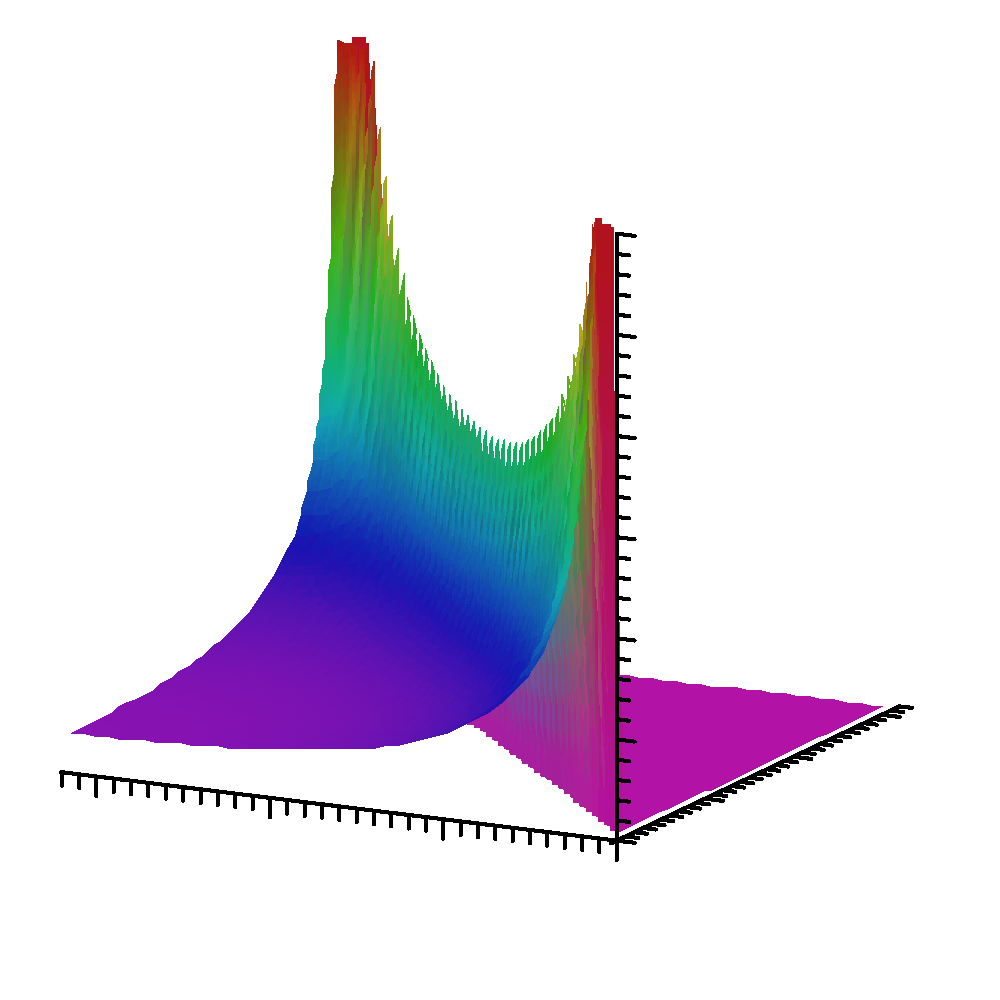
\includegraphics[width=\unitlength]{figures/observabilite.pdf}}%
    \put(0.91898958,0.27276875){\makebox(0,0)[lb]{\smash{$\frac{\pi}{2}$}}}%
%    \put(0.83121042,0.23039375){\makebox(0,0)[lb]{\smash{1.0}}}%
    \put(0.03147562,0.16682917){\makebox(0,0)[lb]{\smash{$\frac{\pi}{2}$}}}%
%    \put(0.24703125,0.14564167){\makebox(0,0)[lb]{\smash{1.0}}}%
%    \put(0.74040625,0.18801875){\makebox(0,0)[lb]{\smash{0.5}}}%
%    \put(0.4195625,0.12445417){\makebox(0,0)[lb]{\smash{0.5}}}%
    \put(0.60262708,0.10326667){\makebox(0,0)[lb]{\smash{0.0}}}%
%    \put(0.65262708,0.14564167){\makebox(0,0)[lb]{\smash{0.0}}}%
    \put(0.63749375,0.24855417){\makebox(0,0)[lb]{\smash{10}}}%
    \put(0.63749375,0.35146667){\makebox(0,0)[lb]{\smash{20}}}%
    \put(0.63749375,0.45135208){\makebox(0,0)[lb]{\smash{30}}}%
    \put(0.63749375,0.5512375){\makebox(0,0)[lb]{\smash{40}}}%
    \put(0.63749375,0.65415){\makebox(0,0)[lb]{\smash{50}}}%
    \put(0.63749375,0.75403542){\makebox(0,0)[lb]{\smash{60}}}%
    \put(0.725,0.65){\color[rgb]{0,0,0}\makebox(0,0)[lb]{\smash{$\tau$}}}%
    \put(0.25777756,0.09570526){\color[rgb]{0,0,0}\makebox(0,0)[lb]{\smash{$\iD$}}}%
    \put(0.83914815,0.17431824){\color[rgb]{0,0,0}\makebox(0,0)[lb]{\smash{$\iT$}}}%
  \end{picture}%
\endgroup
